\documentclass[numbers=noenddot,12pt,a4paper]{scrartcl}
\usepackage[greek,ngerman]{babel}
\usepackage[T1]{fontenc}
\usepackage[utf8]{inputenc}
\usepackage{fullpage}
\usepackage{libertine}
\usepackage{ziffer}
\usepackage{graphicx}
\usepackage{units}
\usepackage[infoshow]{tabularx}
\usepackage{amsmath}
\usepackage{amssymb}
\usepackage{wrapfig}
\usepackage{esint}
\usepackage{float}
\usepackage{wrapfig}
\usepackage[font=small]{caption}
\usepackage{subcaption}

\renewcommand{\thefigure}{Abb. \arabic{figure}}

\captionsetup[wrapfigure]{name=}
\captionsetup[figure]{name=}
\newcommand{\degree}{^\circ}
\newcommand{\diff}{\textnormal{d}}
\newcommand{\tenpo}[1]{\cdot 10^{#1}}
\newcommand{\greek}[1]{\greektext#1\latintext}
\newcommand{\ix}[1]{_\text{#1}}
\newcommand{\imag}{\mathbf{i}}
\newcommand{\tilt}[1]{\textit{#1}}
\newcommand{\grad}[1]{\textit{grad}\left(#1\right)}
\newcommand{\divergenz}[1]{\textit{div}\left(#1\right)}
\newcommand{\euler}{\mathnormal{e}}
\newcommand{\fett}[1]{\textbf{#1}}

\title{Protokoll: Solarzelle}
\author{Tom Kranz, Philipp Hacker}
\date{\today}

\begin{document}
%\setcounter{page}{2}
%\setcounter{section}{1}
\maketitle
\begin{center}
Betreuer: J. Walowski\\
Versuchsdatum: 4./5.11.2014\\
\begin{table}[h]
\centering
Note:
\begin{tabularx}{1.5cm}{|X|}
\hline \\ \\
\hline
\end{tabularx}
\end{table}
\end{center}
\vspace*{\fill}
\tableofcontents
\vfill
\newpage
\section{Einleitung}
Der weltweit 2013 in der Photovoltaik erzeugte Solarstrom reichte aus, um einen Energieverbauch von $\unit[139]{GWh}$ abzudecken. 2008 wurde nach Deutschland mehr Technik für die Photovoltaik importiert, als national hergestellt wurde. Unsere Wirtschaft zählt zu den größten Solarmodulproduzenten weltweit. Vor bereits 4 Jahren lag die in Deutschland \tilt{installierte Leistung} bei $\unit[9760]{MW}$. Die Bedeutung der Solarzelle im Hinblick auf die aktuelle Energiesituation wächst somit ständig an. \\
In diesem Versuch sollen die Eigenschaften einer Silizium-Solarzelle untersucht werden. Es handelt sich hierbei um ein aktives, dotiertes Halbleiter-Bauelement, welches seine Charakteristiken je nach der Intensität und Energie der Beleuchtung verändert. Im speziellen geht es dabei um die Umwandlung von Strahlungsenergie in elektrische Energie über den \tilt{inneren photoelektrischen Effekt}.
\section{Physikalische Grundlagen}
\subsection{Silizium als Halbleiter}
Silizium besitzt 4 Valenzelektronen, welche im Festkörper spingekoppelte, kovalente Bindungen mit Nachbaratomen ausbilden. Die Elementarzelle des \textbf{Si} bildet einen Tetraeder, wobei die Kantenlänge der Zelle und somit die Gitterkonstante des Kristalls $a\ix{Si}=\unit[5,43\cdot 10^{-10}]{m}$ beträgt. Dieser kleinste wiederkehrende Würfel enthält 8 \textbf{Si}-Atome.\\
Halbleiter charakterisieren sich allgemein durch eine Lücke $\Delta E$ zwischen den Energiezuständen ihrer Valenzelektronen. Für $T=\unit[0]{K}$ sind Halbleiter Isolatoren, da ihre \tilt{Bandlücke} zu groß wird und die Valenzelektronen nicht die Energie besitzen, diese \tilt{verbotene Zone} zu überwinden. Für $T>\unit[0]{K}$ können einige dies jedoch, wobei sie Defektelektronen (\tilt{Quasiteilchen}) hinterlassen. Aus dem Valenzband von Nachbaratomen gelöste Teilchen können damit rekombinieren, womit ein Ladungsstrom aus den positiven Quasiteilchen der "`Löcher"' und den angeregten Elektronen entsteht. \fett{Si} wird zum elektrischen Leiter.\\
Der Rekombinationsprozess erfolgt außerdem unter der Abgabe von Impuls an das Kristallgitter. Die daraus resultierende Gitterschwingung kann ebenso durch die Emission eines weiteren \tilt{Quasiteilchens}, des Phonons, dargestellt werden. Diese sind für den Ladungsstrom jedoch irrelevant.\\
In Halbleitern ist die verbotene Zone also klein genug, dass Wärmeschwingungen (auch Lichtabsorption) ausreichen, damit Valenzelektronen angeregt und in ihrem Niveau angehoben werden können. Das heißt: Halbleiter haben eine intrinsische  elektrische Leitfähigkeit.\\
Sei nun die bei einer Temperatur $T$ vorliegende Dichte von negativen bzw. positiven Ladungsträgern $\eta$ und $\rho$, sowie die Beweglichkeit der jeweiligen Teilchen $\mu_\eta$ und $\mu_\rho$. Dann gilt für die Leitfähigkeit $\sigma$:
\begin{align*}
    \sigma=&\mathnormal{e}\cdot\left(\eta\cdot\mu_\eta+\rho\cdot\mu_\rho\right)
\end{align*}
($\mathnormal{e}$ - Elementarladung). Schließlich lässt sich auch die Dichte $n$ der zur Leitung beitragenden, quasifreien Elektronen berechnen. Hierzu benutzt man die \tilt{Fermi-Verteilung} $f(\varepsilon)$ für eine Energie der Teilchen $E_{e^-}=E\ix{Leitung}+\varepsilon$. Es folgt für die $n$ und die Zustandsdichte $N$:
\begin{align*}
	n=4\pi\left(\frac{2m_e}{h^3}\right)^{\frac{3}{2}}\cdot \int_{0}^{\infty}f(\varepsilon)\sqrt{\varepsilon}\diff\varepsilon=2\left(\frac{2\pi m_e k_B T}{h^2}\right)^{\frac{3}{2}}\cdot\euler^{\left(-\frac{\Delta E}{2k_B T}\right)}=N\cdot\euler^{\left(-\frac{\Delta E}{2k_B T}\right)}
\end{align*}
($m_e$ - Elektronenmasse; $h$ - Planck-Konstante, $k_B$ - Boltzmann-Konstante). Im undotierten Halbleiter gilt im Allgemeinen für die Eigenleitungsdichte $n=n\ix{i}=n\ix{Leitung}=n\ix{Defekt}\,$.
\subsubsection{Dotiertes Silizium}
Bringt man in den Festkörper des Silizium Fremdatome mit $k\neq4$ Valenzelektronen, so verändern sich die Bandlücke und Fermi-Energie $E_F$ dahingehend, dass sie sich je nach Wert von $k$ verkleinern oder vergrößern. Dies entspricht der künstlichen Veränderung der Dichten $\eta$ bzw. $\rho$ durch Einbringen von "`Löchern"' mit Akzeptoren oder Elektronen mit Donatoren (zBsp.: $k=5$ \fett{As}; $k=3$ \fett{Al}). Für $k=5$ liegt n-dotiertes Material vor und $E_F$ steigt. Mit $k=3$ sinkt für p-dotiertes Silizium  die Fermi-Energie. Das Quadrat der Eigenleitungsdichte $n\ix{i}$ ist in jedem Fall gleich groß. \\
Die durch die Temperaturbewegung und den Unterschied in den Energien auftretenden Potentialdifferenz lässt sich durch 2 Spannungen ausdrücken: $U\ix{T}$ und $U_{\Delta E}\,$. Für Silizium ist $\Delta E=\unit[1,12]{eV}$. Die Ladungsträgerdichte lässt sich damit umschreiben.
\begin{align*}
		U_{\Delta E}=\frac{\Delta E}{e} \hspace{1cm}&\hspace{1cm} U\ix{T}=\frac{k_B T}{E} \\
		n=N(T)\cdot &\euler^{-\left(\frac{U_{\Delta E}}{2 U\ix{T}}\right)}
\end{align*}
\begin{wrapfigure}[21]{lo}{0.42\textwidth}
	\centering
	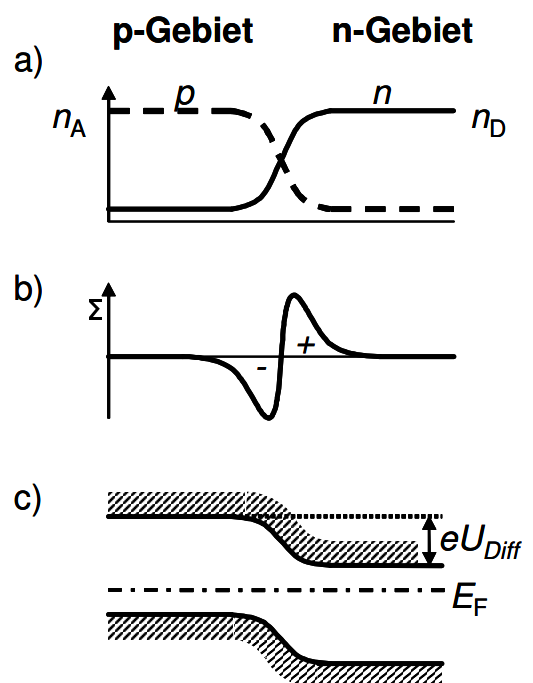
\includegraphics[width=0.4\textwidth]{sigma.png}
	\caption{a) Konzentrationen\\ b) Übergang\\ c) Bänder-"'Knick"'} \label{img:sigma}
\end{wrapfigure}
An einem Übergang von p- zu n-dotiertem Material (und entgegengesetzt) stellt sich ein Diffusionsstrom ein, da der Gradient der jeweiligen Ladungskonzentrationen $n_{\eta}$ und $n_\rho$ nicht null ist. Das heißt, dass ein Konzentrationsgefälle für das "`Wandern"' von Elektronen und Löchern entgegen des jeweiligen Gradienten verantwortlich ist. \\
Die von der Diffusion erzeugten Raumladungszone der Ladung $\Sigma$ (siehe \ref{img:sigma})- Elektronen hinterlassen Defekte und umgekehrt - bauen ein elektrisches Feld auf, welches der Ursache entgegenwirkt. Die Größe des Übergangs kann somit im thermischen Gleichgewicht nicht beliebig anwachsen. Die beschriebene Diffusionsspannung wird folgendermaßen eingeschränkt:
\begin{align*}
	U\ix{L}\leq U\ix{Diff}=U\ix{T}\ln\left(\frac{n_\eta\cdot n_\rho}{n\ix{i}^2}\right)\leq U_{\Delta E}
\end{align*}
Hierbei ist $U\ix{L}$ die maximale Spannung die anliegt, wenn kein Verbraucher an der Solarzelle angeschlossen ist.
\subsection{Funktionsweise der Solarzelle}
Durch Absorption von elektromagnetischer Strahlung werden im Halbleiter freie Ladungsträger erzeugt (innerer Photoeffekt). Durch das von den pn-/np-Übergängen erzeugte innere elektrische Feld sorgt dafür, das es einen gerichteten Ladungsstrom gibt.\\
Minoritätsladungen aus einer dünnen, absorbierenden Siliziumschicht können in die darunterliegende Raumladungszone eines Übergangs diffundieren. Das dort vorliegende Feld trennt diese von den Majoritätsladungen der Absorptionsschicht. Dadurch entsteht ein Strom von, aus der sogenannten Basis diffundierten, Elektronen zwischen den Kontakten der in Reihe geschalteten Übergänge. Die damit einher gehende Spannung ist die Leerlaufspannung $U\ix{L}$. Ein Teil der Diffusionsladungen rekombiniert noch bevor sie zum Strom beitragen können. Die freiwerdende Energie äußert sich durch Erwärmung der Zelle. 
\subsubsection{Qualität einer Solarzelle}
Die Leistung einer Solarzelle hängt natürlich, neben den externen Faktoren, auch von ihrem internen Aufbau und damit ihrer Charakteristik als elektrisches Bauteil ab. Es können geeignete Größen für genau diesen Zweck eingeführt werden. Der Füllfaktor \fett{FF} ist das Verhältnis aus maximaler Leistung zum Produkt aus $U\ix{L}$ und $I\ix{Photo}$ (siehe \ref{img:detail}). Als Spannungsfaktor \fett{SF} bezeichnet man den Quotienten aus $U\ix{L}$ und $U_{\Delta E}$. Das Produkt von beiden ergibt schließlich den charakteristische Faktor \fett{CF}.
\subsubsection{Strom-Spannungscharakteristik}
\begin{wrapfigure}[10]{ro}{0.39\textwidth}
	\centering
	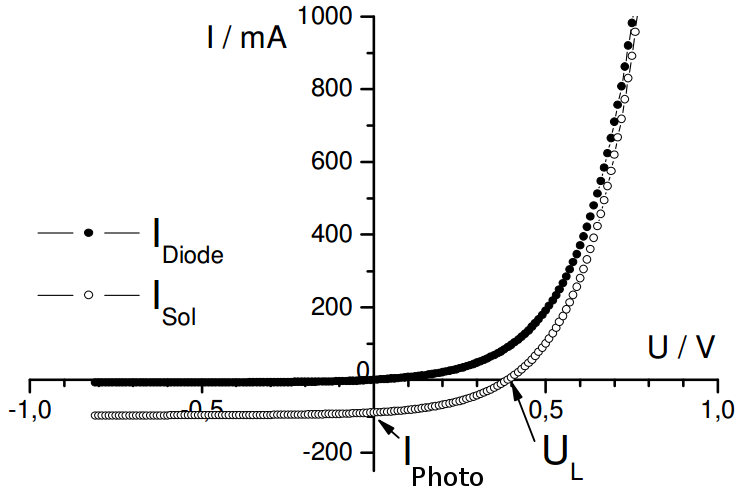
\includegraphics[width=0.39\textwidth]{strom.png}
	\caption{Vergleich Diode-Solarzelle} \label{img:strom}
\end{wrapfigure}
Eine Solarzelle ist eine (Photo-)Diode, welche aufgrund des inneren Photoelektrischen Effektes aus elektromagnetischer Strahlung einen gerichteten Strom erzeugt. Der Strom der Zelle kann genähert als Summe aus einem Strom durch das Bauteil Diode $I\ix{D}$ und einen von der Leerlaufspannung getriebenen Strom $I\ix{Photo}$ betrachtet werden (siehe \ref{img:strom}).
\begin{align*}
	I\ix{Sol}=&I\ix{D}-I\ix{Photo} \\
	I\ix{D}=I\ix{sat}\euler^{\left(\frac{U}{U\ix{T}}-1\right)} \hspace{0.75cm}&\hspace{0.75cm} I\ix{Photo}=\eta\ix{Photo}\cdot\frac{\lambda \mathnormal{e}}{h\cdot c}\cdot P\ix{opt}
\end{align*}
($I\ix{sat}$ - Sättigungsstrom; $P\ix{opt}$ - optische Leistung; $E=\frac{hc}{\lambda}$ - eingestrahlte Energie; $\eta_{opt}$ - Wirkungsgrad) \\
Unbeleuchtet folgt der Strom-Spannungsverlauf der Solarzelle dem einer Diode (siehe \ref{img:strom}). Beleuchtet man hingegen eine unbeschaltete Zelle, so sieht man $I\ix{sol}(U\ix{L})=0$ wegen der Aufladung der Ladungszonen der dotierten Gebiete.\\
Schließt man die Solarzelle kurz und beschaltet sie mit einem Signal $U\neq0$, so rekombinieren die Ladungen des Signals und des Leerlaufstroms miteinander. Die $U$-$I$-Kennlinien der Diode und der Solarzelle gleichen sich damit im Betrieb an.\\
Für den Photo-Strom gilt, das sowohl die Photonenenergie als auch der Wirkungsgrad von der Wellenlänge abhängen. Offensichtlich muss, aufgrund der Quantisierung der Energien für die Zustände und der Photonen $E\ix{opt}\geq\Delta E$ gelten.
\begin{figure}[h]
	\centering
	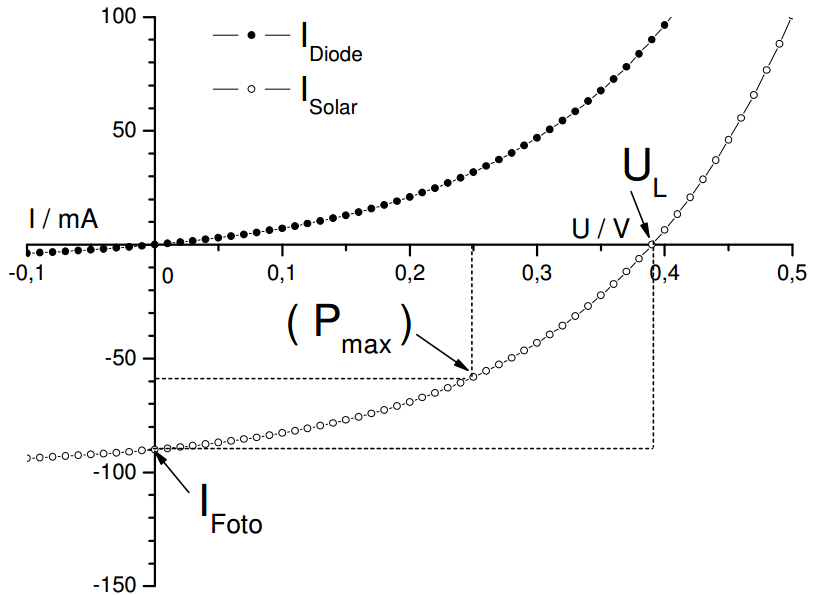
\includegraphics[width=0.65\textwidth]{detail.png}
	\caption{maximale Leistung und Photo-Strom der Solarzelle} \label{img:detail}
	\end{figure}
\section{Durchführung}
Mit Hilfe von Spannungs- und Strommessgeräten wird eine einfache Solarzelle untersucht.\\
Eingangs betrachtet man das unbeleuchtete Bauteil. Durch eine externe Spannungsquelle wird ein nicht zu großer Bereich von Spannungen generiert und an die Zelle angeschlossen. Der Zusammenhang von Spannung und dem Strom durch den Halbleiter wird aufgenommen. Ebenso wird für Licht verschiedener Farben, Strahler und Intensitäten verfahren.\\
Schließlich bestrahlt man die Solarzelle mit einer $\unit[120]{W}$ Lampe und belastet sie mit Dekaden-Widerständen. Hierbei wird ebenso eine Strom-Spannungscharakteristik verfolgt. Gleiches wird für Tageslicht unternommen.
\section{Auswertung}
\section{Anhang}
Die originalen Messwert-Aufzeichnungen liegen bei.
\end{document}